\documentclass[10pt,twocolumn,letterpaper]{article}

\usepackage{cvpr}
\usepackage{times}
\usepackage{epsfig}
\usepackage{graphicx}
\usepackage{amsmath}
\usepackage{amssymb}

% Include other packages here, before hyperref.

% If you comment hyperref and then uncomment it, you should delete
% egpaper.aux before re-running latex.  (Or just hit 'q' on the first latex
% run, let it finish, and you should be clear).
\usepackage[pagebackref=true,breaklinks=true,letterpaper=true,colorlinks,bookmarks=false]{hyperref}

\cvprfinalcopy % *** Uncomment this line for the final submission

\def\cvprPaperID{****} % *** Enter the CVPR Paper ID here
\def\httilde{\mbox{\tt\raisebox{-.5ex}{\symbol{126}}}}

% Pages are numbered in submission mode, and unnumberesd in camera-ready
\ifcvprfinal\pagestyle{empty}\fi
\begin{document}

%%%%%%%%% TITLE
\title{Data Anomaly Detector - CS 7643}

\author{Lily Chebotarova, Raga Lasya Munagala, Ligeng Peng, Brian Zhang\\
% For a paper whose authors are all at the same institution,
% omit the following lines up until the closing ``}''.
% Additional authors and addresses can be added with ``\and'',
% just like the second author.
% To save space, use either the email address or home page, not both
Georgia Institute of Technology\\
{\tt\small lily.chebotarova@gmail.com, rmungala6@gatech.edu, kevinplg@gatech.edu, brianxicheng@gmail.com}
}

% \author{Lily Chebotarova\\
% {\tt\small lily.chebotarova@gmail.com}\\
% \and 
% Raga Lasya Mungala\\
% {\tt\small rmungala6@gatech.edu}\\
% \and 
% Ligeng Peng\\
% {\tt\small kevinplg@gatech.edu}\\
% \and 
% Brian Zhang\\
% {\tt\small brianxicheng@gmail.com}\\
% }

\maketitle
% \thispagestyle{empty}

%%%%%%%%% ABSTRACT
\begin{abstract}
   Anomaly detection is an important and prevalent problem across multiple domains, such as credit card fraud, medical diagnostics, and many others. 
   Existing common approaches applied to anomaly detection often consist of supervised machine learning such as clustering or ensemble methods like random forest.
   These approaches often have limitations in their ability to learn complexities of anomalous data structures.
   In this project, we examine leading papers describing novel methods in the field of anomaly detection for timeseries data. We reproduce the results of these
   papers while ekeing out additional performance by fine-tuning of the models when applied to an established labelled dataset for anomaly detection, "S5- A Labeled Anomaly Detection Dataset". 
   The first method examined is a Convolutonal-Long-Short-Term-Memory (C-LSTM) neural network, as described in the paper by Tae-Young Kim and Sung-Bae Cho \cite{kim2018web}.  
   Model performance similar to that of the authors is demonstrated using a pytorch implementation of the model architecture described. 
   We also achieve similar performance with an autoencoder architecture proposed by several papers in the anomaly detection field \cite{hagemann2020reconstruction, wong2022aer}.
\end{abstract}

%%%%%%%%% BODY TEXT
\section{Introduction/Background/Motivation}

Anomalies represent some sort of irregularity in the normal pattern or the prevailing trend of data, or in other words they are data points that stand out from the others 
and deviate from observed and expected behavior in the data. Anomalies can include outliers, drifts in data or other changes in the system. Perhaps the most common type of 
anomaly detection problem, and the type addressed by this paper, occurs in time series data. Anomaly detection is a common problem across many domains, with potentially profound 
implications if addressed effectively. The ability to accurately identify anomalies enables proactive detection of irregular patterns, diagnostic of potential issues, and enhancement 
of the quality and reliability of various services. Anomalies in web-traffic data may indicate potential issues such as unexpected spikes in user traffic which may be due to 
cyber-attacks, system failures, or viral trends. 

(5 points) How is it done today, and what are the limits of current practice?
The current state of the art in timeseries anomaly detection primarily consists of deep learning methods, which together with the high prevalence and importance of this problem, makes it an 
ideal candidate for study in this paper. Deep Learning methods have been found to significantly outperform the more traditional methods, as they are able to learn hierarchical features and capture 
complexities in the data and perform better at large scale \cite{chalapathy2019deep}. Common deep learning methods employed in this field include Long Short-Term Memory (LSTM) networks and autoencoders, both of which we 
examine in this paper. RNN-based methods such as these are particularly well-suited for timeseries problems which inherently consist of sequential data \cite{chalapathy2019deep}. Autoencoders have also been successfully 
applied to time-series anomaly detection in unsupervised scenarios and performed better than methods such as Local Outlier Factor and Principal Component analysis \cite{hagemann2020reconstruction}.

Our paper examines leading novel approaches in this field of anomaly detection and compares the relative performance of these methods. Our paper examines leading novel approaches in this field of anomaly detection and compares 
the relative performance of these methods. The first method examined is C-LSTM neural network applied to time series web traffic data, as described in the paper by Tae-Young Kim and Sung-Bae Cho \cite{kim2018web}. 
Model performance similar to that of the authors is demonstrated using a pytorch implementation of the model architecture described. The second method reproduced is an autoencoder approach, as
described in the paper by Lawrence Wong, et al \cite{wong2022aer}.

The paper by Tae-Young Kim and Sun-Bae Cho \cite{kim2018web} offers an improvment over conventional LSTM approaches by integrating a convolutional layer as the input for LSTM layer, reducing temporal variations 
and improivng overall performance. Similarly, the paper by Lawerence Wong, et al. \cite{wong2022aer} offers an improvment over conventional approaches by combining separate autoencoder and LSTM approaches models into 
a single composite model optimizing a joint objective function, and able to make bi-directional predictions. We will compare the effectiveness of the two approaches investigated in this paper to see 
which offers the best performance on the anomaly detection dataset selected.

We will compare the effectiveness of the two approaches investigated in this paper to see which offers the best performance on the anomaly detection dataset selected. Timely detection of these anomalies is essential for organzing a prompt response and minimizing the impact to system performance and user experience. 
In short, a robust and effective anomaly detection method for a given problem should allow us to proactively detect irregular patterns and diagnose potential issues, thus
enhancing the quality and reliability of the services tracked by this timeseries data. 

Our paper uses the dataset, S5 A Labeled Anomaly Detection Dataset \cite{yahooS5}, which offers a diverse range of real and synthetic time-series data specifically curated for the purpose of anomaly detection. 
The dataset is publicly available via Yahoo Research \cite{yahooS5}. This dataset was chosen because it offers a diverse set of edge cases for testing our models, including outliers and various change-points. 
The time series data also includes varying trend, noise, and seasonality which enables us to better test the robustness of our model implementations. 
The real portion of the dataset is made up of the web traffic metrics of various yahoo services, alongside synthetic data added to the dataset.

%-------------------------------------------------------------------------
%------------------------------------------------------------------------
\section{Approach}

\subsection{Pre-processing}
First, we applied pre-processing steps and exploratory analysis to the data. We focused on the A1 part of the Yahoo dataset that consists of the real web 
traffic with manual human-applied labels for anomalies. It is presented in 67 separate files with traffic measures from various Yahoo web services and anomaly 
data. The data in this dataset is represented by a time series of traffic measurement values from actual web series in one hour units. 
Since the labeling was manually done, there is potential for some inconsistency in data.The traffic also presents a high level of variability.  
The data from 67 files was concatenated for training, values were normalized and any values in traffic data that were equal to zero were dropped. 
Normalizing data was important as it ensured that we didn’t have features with larger scales or variances that could dominate the learning process. 
The values were normalized using the Euclidean norm. This was achieved using the preprocessing.normalize function available in scikit-learn in Python. The resulting normalized has each row scaled such that the Euclidean norm (the square root of the sum of squares of each element) of each row is 1. 
The normalized web-traffic timeseries data is shown in Figure \ref*{pre-process-web-traffic}. 

\begin{figure}[ht]
   \centering
   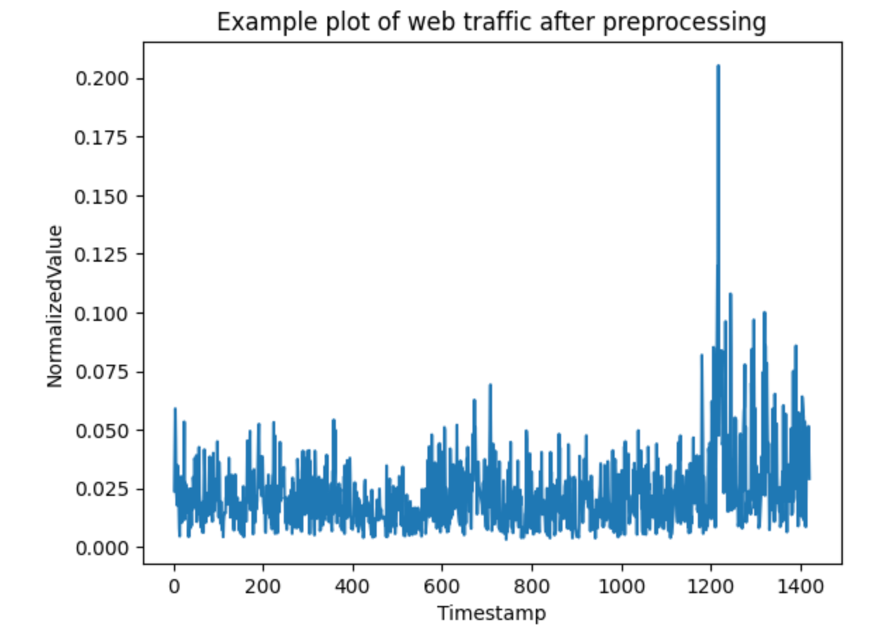
\includegraphics[width=0.5\textwidth]{images/webtraffic.png}
   \caption{Pre-processed Web Traffic Timeseries Data}
   \label{pre-process-web-traffic}
   \end{figure}

The structure of the problem is characterized by a highly imbalanced dataset, with normal network activity dominating and anomalies representing a minority class.  Considering these characteristics of the data, we employed the sliding window method to the data.
In this sliding window technique, we created  windows of data by sliding a fixed-size window across the data samples. For the data presented in this dataset, we created a sliding window of length 60. 

To perform anomaly detection on the preprocessed dataset, we trained and evaluated an Autoencoder and C-LSTM network. We also further compared the performance to traditional machine learning methods such as Random Forest. 

In response to addressing the highly imbalanced nature of the dataset, we have innovatively incorporated a sliding window methodology as part of our preprocessing strategy. This approach entails 
carefully segmenting the dataset into distinct windows, allowing for a more balanced representation of both normal and anomaly instances. By implementing this sliding window technique, we aim to 
mitigate the inherent imbalance and create a more equitable distribution of data points, fostering a robust learning environment for our model. This comprehensive evaluation involves comparing the 
performance of our model across different preprocessing strategies to discern the most effective approach for anomaly detection.

\subsection{Autoencoder}
The structure of the autoencoder model was designed to reflect the underlying imbalanced makeup of the dataset.
We start the problem with 70\% training dataset and 30\% testing dataset. The encoder is trained on a subset of the training dataset, capturing the essential characteristics of the network traffic, before being trained 
per the following steps:

\begin{enumerate}
    \item Created an autoencoder with an encoder and a decoder in PyTorch.
    \item Trained the autoencoder using the training dataset.
    \item Extracted the encoder from the trained autoencoder.
    \item Built a classifier using the extracted encoder for feature representation.
    \item Trained the classifier using the features from the training set.
    \item Evaluated the model on a separate test set, passing inputs through the autoencoder and then through the classifier, calculating accuracy for anomaly detection.
\end{enumerate}

In the autoencoder model, the parts with learned parameters were primarily associated with the encoder and decoder components. These components consisted of linear layers (fully connected) 
and activation functions, such as ReLU, designed to transform and compress the input data. Specifically, the encoder learned to map the input features to a lower-dimensional representation, 
capturing essential information about normal network behavior. Conversely, the decoder learned to reconstruct the input data from this compressed representation \ref*{autoenc-network}

The post-processing classifier, which was applied for decision-making or anomaly identification, involved a separate linear layer followed by a sigmoid activation function. This part of the model 
facilitated the conversion of the encoded features into decision probabilities, determining whether a given input represented normal or anomalous network activity. While the weights of the linear 
layer in the post-processing step were learned during training, this part of the model served more as a decision-making component than a feature extraction one.

\begin{figure}[ht]
   \centering
   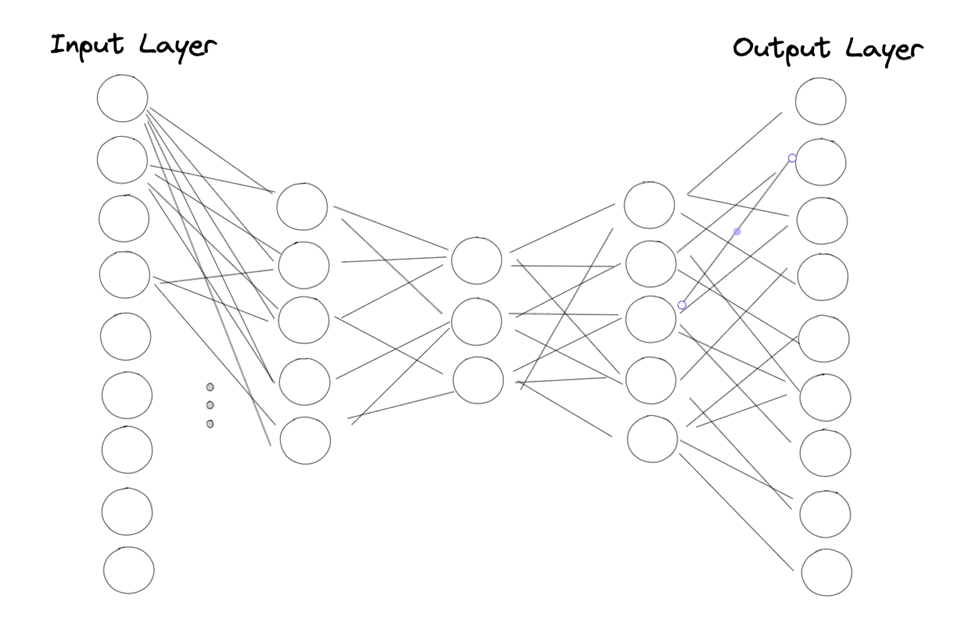
\includegraphics[width=0.5\textwidth]{images/autoenc-network.png}
   \caption{Autoencoder-Decoder Diagram}
   \label{autoenc-network}
   \end{figure}

In the quest to optimize the autoencoder model, several hyperparameters were explored and fine-tuned to enhance overall performance. The initial architecture, characterized by three linear layers in both 
the encoder and decoder with hidden dimensions (16, 8, 4), underwent significant adjustments. The optimized architecture featured larger hidden dimensions in the encoder (64, 32, 16) and a mirrored structure 
in the decoder (16, 32, 64). This architectural refinement aimed to empower the model with the capacity to capture more intricate patterns within the data. Moreover, the learning rate, a critical factor 
influencing training dynamics, was systematically tested at values of 0.001, 0.005, and 0.01. Through careful evaluation, a learning rate of 0.005 emerged as the most effective in striking a balance 
between convergence speed and stability.

Batch size, another crucial hyperparameter, was subjected to experimentation with various sizes. The optimal batch size was identified as 512, showcasing its pivotal role in facilitating efficient model 
training and convergence. Furthermore, the choice of optimizer played a significant role in the training process. The Adam optimizer was selected for its effectiveness in optimizing neural networks, 
contributing to the overall success of the model.
In our initial attempt to model the data directly, we encountered a significant challenge due to the highly imbalanced nature of the dataset. 
Despite achieving an impressive overall accuracy of 98.15\%, the F1 score, a critical metric for evaluating model performance, remained notably low at 13\%. This low F1 score suggested that the model 
struggled to discern and learn the essential patterns or features crucial for accurate predictions.
Recognizing the limitations of our first approach, we pivoted to employ the sliding window method. This strategic adjustment proved instrumental in addressing the imbalance issue and yielded 
tangible improvements, particularly in the F1 score. The sliding window method allowed for a more nuanced analysis of the data, contributing to a refined understanding of the underlying patterns. 
Consequently, our model exhibited enhanced performance, showcasing the importance of tailored preprocessing techniques in handling imbalanced datasets and improving overall predictive accuracy.


\subsection{C-LSTM}
The C-LSTM model is particularly well-suited for anomaly detection in time series data due to its unique architecture that combines the strengths of convolutional neural networks (CNNs) and 
long short-term memory networks (LSTMs). Real web traffic data with manual anomaly labels presented in the Yahoo data set has patterns of spatial and temporal information. LSTMs are traditionally an 
effective choice for anomaly detection especially on sequential data due to their ability to extract temporal features of the data. Additionally, the ability of these models to capture long-term dependencies 
in time-series data also makes them more adaptable to evolving data patterns, which is crucial for accurately identifying anomalies over time. Further, the CNN layers provide the benefit of reduction of 
variation in spatial information.  This combination allows the model to effectively capture both spatial and temporal features in the data, which are crucial for accurately identifying anomalies \cite{kim2018web} to 
achieve higher performance for anomaly detection in time series. We attempt to replicate the results of the model presented in the paper by Tae Young Kim, Sung Bae Cho \cite{kim2018web}.

The data was pre-processed using the sliding window approach, with the length of the web traffic window set to 60.Our model was built in PyTorch as opposed to Keras model presented in the paper, 
with architecture presented in Table 1. First, there are 2 convolutional layers, each followed by the tanh activation and max pooling. Then the LSTM is applied to extract the temporal features from the data. 
Finally, two fully-connected linear layers and softmax are applied for the final classification task and output layer. We noticed differences in behavior of the model in Pytorch as compared to Keras model, 
which can potentially be explained by the underlying differences in how these frameworks handle certain factors in the model architecture and training, like weight initialization, loss functions etc. 
Due to some of these differences, the total number of parameters and certain attributes have been modified for Pytorch implementation. Additionally, gradient clipping was implemented to prevent exploding 
gradients. 

\subsection{Hyperparameter Tuning}
As part of optimizing the C-LSTM and autoencoder models, we employed a detailed hyperparameter tuning framework designed to optimize the performance of both Convolutional Long Short-Term Memory (C-LSTM) 
and Autoencoder models. This framework is pivotal in determining the most effective configurations for our models, ensuring they are finely tuned for the specific tasks of feature 
representation and anomaly detection. We adopted a systematic approach to explore a wide range of hyperparameters, including but not limited to, layer dimensions, learning rates, and activation functions. 
The range of tuning parameters for the C-LSTM and Autoencoder models are shown is shown in Figure \ref*{clstm-tuning-matrix} and Figure \ref*{autoenc-tuning-matrix}, respectively.

\begin{table}[h]
   \centering
   \caption{Hyperparameter tuning grid for C-LSTM model}
   \label{clstm-tuning-matrix}
   \begin{tabular}{|l|l|}
   \hline
   \textbf{Hyperparameter}   & \textbf{Values}         \\ \hline
   Conv1 Output Channels     & 16, 32                  \\ \hline
   Kernel Size               & 3, 5                    \\ \hline
   LSTM Hidden Size          & 16, 32                  \\ \hline
   FC1 Output Features       & 4, 16, 32               \\ \hline
   Learning Rate             & 0.001, 0.01             \\ \hline
   Optimizer                 & Adam             \\ \hline
   Criterion                 & BCELoss                 \\ \hline
   Epochs                    & 200                     \\ \hline
   \end{tabular}
   \end{table}

\begin{table}[h]
      \centering
      \caption{Hyperparameter tuning grid for Autoencoder model}
      \label{autoenc-tuning-matrix}
      \begin{tabular}{|l|l|}
      \hline
      \textbf{Hyperparameter}               & \textbf{Values}                                 \\ \hline
      Encoder Layer Sizes                   & \small{[32,16,8],[64,32,16],[128,64,32]}       \\ \hline
      \small{Autoencoder Learning Rate}           & 0.001, 0.01, 0.05                               \\ \hline
      \small{Classifier Learning Rate}            & 0.0005, 0.001, 0.005                            \\ \hline
      Activation                            & LeakyReLU, ReLU                                 \\ \hline
      Optimizer                             & Adam                                            \\ \hline
      Criterion                             & MSELoss                                         \\ \hline
      Epochs                                & 200                                             \\ \hline
      \end{tabular}
      \end{table}

For the C-LSTM model, hyperparameter tuning focused on its unique architecture that combines convolutional layers with LSTM units. 
Key hyperparameters include the number and size of convolutional filters, kernel sizes, the number of LSTM units, and the architecture of fully connected layers. 
Given the sequential nature of our data, special attention was given to the size of the LSTM units, which play a crucial role in capturing temporal dependencies.
The convolutional layers were fine-tuned to effectively extract spatial features before they were fed into the LSTM units. The learning rate was also 
adjusted to balance the speed and stability of the training process.

For the autoencoder tuning focused on the encoder and decoder's layer sizes and the activation functions used. The depth and breadth of these layers were 
especially important in determining the model's ability to compress and reconstruct the input data effectively. The leaky ReLU actiation function was tested
in addition to the original ReLU activation, as it was hypothesized that outliers we are seeking to focus on in an anomaly detection problem may be better 
represented by allowing a small gradient for negative values (over the dead-neurons at the zero-cutoff for ReLU).


\section{Experiments and Results}
The dataset we had is highly imbalanced. It's important to note that while the accuracy metric is commonly used, its reliability can be 
compromised in the presence of imbalanced datasets. For instance, if anomalies are significantly outnumbered by normal cases, a high overall 
accuracy may be misleading. In the context of anomaly detection, the actual detection of anomalies becomes crucial.
In this scenario, precision, recall, and F1-score metrics can provide a more nuanced evaluation of the model's performance. 
Precision evaluates the accuracy of positive predictions, recall assesses the model's ability to capture all actual positives, and the F1-score 
balances precision and recall. These metrics are particularly useful for addressing class imbalance and providing a more comprehensive understanding of 
the model's strengths and weaknesses.

For our experiment, the best hyperparameters for each model were selected as the set yiel
\subsection{Experiments}

Throughout the development of the autoencoder model for anomaly detection, a series of experiments were systematically conducted to address various challenges and 
enhance the model's overall performance. Given the highly imbalanced nature of the initial dataset, the effectiveness of different techniques, such as the sliding window 
method and subsampling, was thoroughly explored to balance the dataset and improve the model's ability to detect anomalies. Additionally, hyperparameter tuning played a 
crucial role in optimizing the model. The architecture of the autoencoder, including the number of layers and neurons per layer, as well as hyperparameters like the learning 
rate and batch size, were systematically adjusted and tested to identify the most effective configuration. The training process involved monitoring the loss function over 100 
epochs, ensuring convergence and assessing the model's learning progress.

In conjunction with the autoencoder, a classifier was trained on the encoded features to perform binary classification. The training of this classifier was evaluated over 
multiple epochs to gauge its effectiveness in distinguishing between normal and anomalous instances. Quantitative evaluation experiments included the calculation of various 
metrics such as accuracy, precision, recall, and F1-score on a separate test set. These metrics provided valuable insights into the model's ability to correctly classify 
instances and handle class imbalances effectively. Finally, the performance of the autoencoder model was compared with other models, such as a Random Forest classifier, to 
assess its relative effectiveness in anomaly detection. Through these comprehensive experiments, the iterative refinement of the model aimed to overcome challenges, optimize 
its architecture, and achieve accurate anomaly detection.

\subsection{Results}
While the quantitative results indicate a decrease in the reconstruction loss, a qualitative analysis involves inspecting the reconstructed outputs visually or through 
other means. The loss function used in the provided code is the Mean Squared Error (MSE) loss. The MSE loss is computed between the reconstructed outputs (outputs) 
generated by the autoencoder and the original inputs (inputs). It measures the average squared difference between corresponding elements of these two tensors. 
The criterion variable, which is used to calculate the loss, is initialized as nn.MSELoss() earlier in the code. The model then minimizes this loss during training to 
improve the reconstruction performance and learn a meaningful representation of the input data.

The progression from an initial loss of 0.4728 to a final loss of 0.1211 highlights the effectiveness of the Autoencoder in minimizing the dissimilarity between the 
original and reconstructed data. This trend suggests that the model has successfully captured meaningful representations of the input features, resulting in a more 
refined and optimized reconstruction of the data. Such a quantitative improvement supports the overall success of the Autoencoder in its learning objectives.
The success of the Autoencoder model can be assessed based on the performance metrics summarized in the results. While the Autoencoder achieved a high accuracy 
of 92.54\%, indicating its ability to make correct predictions on the overall dataset, it is crucial to delve deeper into other metrics for a more comprehensive evaluation.
Precision, recall, and F1-Score provide insights into the model's performance in detecting anomalies specifically. 
The Autoencoder demonstrates a precision of 68.80\%, indicating that when it predicts an anomaly, it is correct approximately 68.80\% of the time. 
However, the recall is 34.16\%, implying that the model may not be capturing all actual anomalies, missing a significant portion.
The F1-Score, which balances precision and recall, is 45.65\%, suggesting a trade-off between correctly identifying anomalies and minimizing false positives.
In summary, while the Autoencoder shows a high overall accuracy, its success in anomaly detection is tempered by a lower recall and F1-Score, indicating room for 
improvement in capturing true anomalies.

\subsection*{Potential Areas for Improvement}
The success of the autoencoder model hinges on its performance in identifying anomalies during the subsequent evaluation phase. 
The effectiveness of anomaly detection will be assessed in conjunction with the classifier's performance.
The dataset exhibits a significant class imbalance, with the majority being normal network instances, while accurate anomaly detection remains crucial. 
Despite our attempt to address this through the window sliding method for balancing the dataset, an alternative strategy involves selectively omitting some normal data. 
This approach aims to enhance accuracy in identifying anomaly data points by mitigating the impact of the dominant normal class.


%-------------------------------------------------------------------------
\begin{table*}
\begin{tabular}{|l|c|p{6cm}|}
\hline
Student Name & Contributed Aspects & Details \\
\hline\hline
Lily Chebotarova            & C-LSTM and initial research  & Researched labelled anomaly detection datasets and found selected Yahoo dataset for project. Developed C-LSTM model implementation code \(anomalydetection.ipynb\). \\ \hline 
Raga Lasya Munagala         & Pre-processing & Developed data pre-processing code \(data\_preprocessing.ipynb\). \\ \hline
Ligeng Peng                 & Auto-encoder with Regression  & Developed autoencoder with regression model implementation code \(anomaly\_detection\_encoder.ipynb\). \\ \hline
Brian Zhang                 & Hyperparamater Tuning, Overall Report and LaTeX  & Performed hyperparameter tuning of both models. Trained final models and evaluated results. Responsible for LaTeX compilation and overall report format/organization. Primary author for abstract, introduction. Created and maintained team git repo: \url{https://github.com/brian-x-zhang/CS7643-Anamoly}. \\ \hline
\hline
\end{tabular}
\caption{Contributions of team members.}
\label{tab:contributions}
\end{table*}


%-------------------------------------------------------------------------


{\small
\bibliographystyle{ieee_fullname}
\bibliography{egbib}
}

\section{Loss}

\end{document}
